
\title{Beschreibung des Prototypen-Content}
\author{apoehlmann}
\date{7.11.2015}

\pdfinfo{%
  /Title    (Beschreibung des Prototypen-Content)
  /Author   (apoehlmann)
  /Creator  (apoehlmann)
  /Keywords (SECH EEXCESS Content Prototyp)
}

\pagebreak

\section{Beschreibung}
Der Content-Prototyp ermöglicht es, Anfragen an den Server des  
\href{https://github.com/EEXCESS/eexcess/wiki}{EEXCESS-Projektes} zu schicken.
Der Prototyp unterstützt das \href{https://github.com/EEXCESS/eexcess/wiki/%5B21.09.2015%5D-Request-and-Response-format#pp-query-format}{PP-QF2}
und somit auch das \href{https://github.com/EEXCESS/eexcess/wiki/%5B21.09.2015%5D-Request-and-Response-format#pp-response-format}{PP-RF2}.

\section{Verarbeiten/Aufbauen der Anfragen}
\subsection{Anfrage}
\begin{enumerate}
  \item Auslesen der Suchbegriffe
    \begin{itemize}
      \item Beachten der Trennung der Suchbegriffgruppen
      \item Einfügen in ein Dictionary, als Schlüssel wird der Suchbegriff genommen
      \item Die Schlüssel werden in die ComboBox für das Bearbeiten der Werte eingefügt
    \end{itemize}
  \item Die Suchbegriffe der Parameter werden bearbeitet (isMainTopic und Type) (optional)
  \item Eingabe der Preferenzen (optional)
  \item Abschicken der Anfrage:
    \begin{enumerate}
      \item Suchwörter, Preferenzen und die generierte QueryID werden an den \href{https://github.com/SECH-Tag-EEXCESS-Browser/iOSX-App/blob/master/Team%20Content/Demos/JSON/Sech/Sech/MainController.swift}{MainController} weitergegeben
      \item Übergabe der Werte an den \href{https://github.com/SECH-Tag-EEXCESS-Browser/iOSX-App/blob/master/Team%20Content/Demos/JSON/Sech/Sech/JSONManager.swift}{JSONManager}
      \item Die Schlüssel werden in die ComboBox für das Bearbeiten der Werte eingefügt
      \item Werte werden in das \href{https://github.com/SECH-Tag-EEXCESS-Browser/iOSX-App/blob/master/Team%20Content/Demos/JSON/Sech/Sech/Json.swift}{JSONObject} eingefügt und zurückgegeben
      \item JSONObject wird über den MainController an den \href{https://github.com/SECH-Tag-EEXCESS-Browser/iOSX-App/blob/master/Team%20Content/Demos/JSON/Sech/Sech/ConnectionManager.swift}{ConnectionManager} weitergegeben
      \item Der ConnectionManager verschickt die Daten an den Server
    \end{enumerate}
  \item Die Antwort vom Server wird im \href{https://github.com/SECH-Tag-EEXCESS-Browser/iOSX-App/blob/master/Team%20Content/Demos/JSON/Sech/Sech/ViewController.swift}{ViewController:53} entgegen genommen und dargestellt
  \item Speichert JSON in das Dictionary "mapOfJSONs" in der Klasse ''MainController''
  \item Fügt die DocumentBages in die die ComboBox für die DetailAnfrage
\end{enumerate}
\pagebreak
\subsection{DetailAnfrage}
    \begin{enumerate}
      \item Auswahl des DocumentBag oder der "take all" Option
      \item Betätigen des "Search Details"-Buttons
	\begin{enumerate}
	  \item Übergibt den DocumentBag/DocumentBags an den JSONManager über den MainController
	  \item JSONObject wird erzeugt und zurückgegeben
	  \item DetailAnfrage wird an den Server übermittelt
	\end{enumerate}
      \item Antwort wird vom ViewController:68 entgegengenommen und im TextFeld dargestellt
    \end{enumerate}
\section{Aufbau des Prototypen}

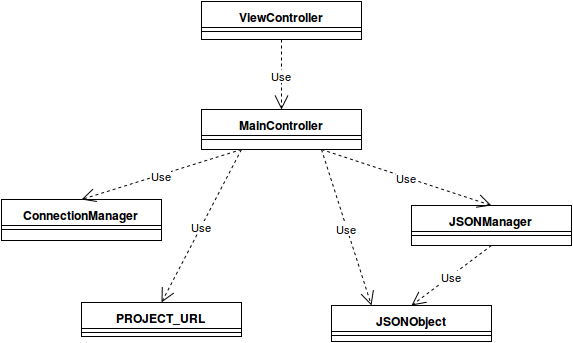
\includegraphics[scale=0.5]{KlassendiagrammContentPrototyp.png}
\pagebreak
\section{JSON}

Der JSON wird in der Klasse \href{https://github.com/SECH-Tag-EEXCESS-Browser/iOSX-App/blob/master/Team%20Content/Demos/JSON/Sech/Sech/Json.swift}{JSONObject} 
gehalten. Ein Dictionary in der Klasse speichert alle Schlüssel/Wert-Paare des JSONObjects.
Es gibt drei Varianten für das Erstellen eines Objekts der Klasse JSONObject:
\begin{itemize}
\item ohne Übergabewert
\item mit einem Dictionary
\item mit einem NSData-Objekt, welches ein Dictionary enthält
\end{itemize}

Die Klasse JSONObject besitzt verschiedene Methoden:
\begin{itemize}
\item Auslesen von Werten (spezialisiert auf bestimmte Datentypen)
\item Einer found()-Methode zum Überprüfen, ob der Schlüssel vorhanden ist
\item Zum Erweitern des JSONs mit Werten
\item Convert-Methoden für das Umwandeln von JSONObject in String und NSData
\end{itemize}

Die Klasse JSONObject kann ohne großen Aufwand um weitere Methoden ergänzt werden, wie zum Beispiel um eine Methode, getImage(key:String) zu erweitern.


\section{Netzwerkverbindungen}

Die Klasse \href{https://github.com/SECH-Tag-EEXCESS-Browser/iOSX-App/blob/master/Team%20Content/Demos/JSON/Sech/Sech/ConnectionManager.swift}{ConnectionManager} ist für das Erstellen einer Verbindung zum Server zuständig. Sie besitzt eine öffentliche Methode ''makeHTTP\_Request''.
 Zusätzlich gibt es eine Klasse \href{https://github.com/SECH-Tag-EEXCESS-Browser/iOSX-App/blob/master/Team%20Content/Demos/JSON/Sech/Sech/ConnectionManager.swift}{PROJECT\_URL} für die URLs, welche im Projekt benötigt werden.

\section{UI}
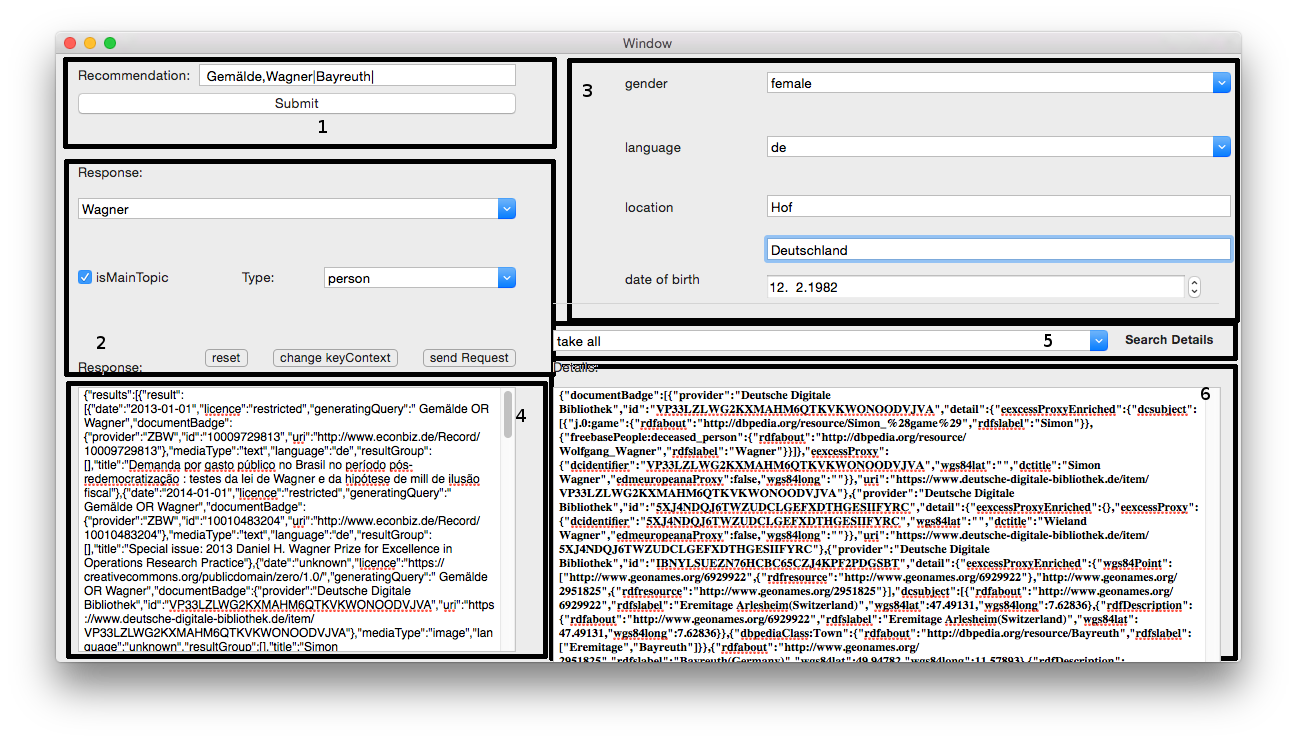
\includegraphics[scale=0.35]{ContentPrototyp2.png}
\begin{enumerate}
\item Eingabe der Suchbegriffe. Mit '','' werden die Begriffe getrennt und mit ''|'' werden die Suchbegriffgruppen getrennt
\item Hier können den Suchbegriffen noch Eigenschaften hinzugefügt werden. Nach jeder Änderung muss der "change keyContext"-Button gedrückt werden. Mit dem Button ''send Request'' wird die Anfrage verschickt. Der Button ''reset'' besitzt keine Funktion.
\item In diesem Bereich können zusätzliche Informationen für die Anfrage angegeben werden.
\item Anzeige der Antwort vom Server
\item Auswahlmöglichkeiten für die Detailanfrage und der ''Search Details''-Button
\item Anzeige der DetailAntwort vom Server
\end{enumerate}

